\section{Architecture}
\label{sec.architecture}


\par
In this section, we describe the design and architecture of Lind. We explain the choices we made and the rationale behind our decision. We also discuss the challenges we are facing.


\par
The primary goal of Lind is to execute untrusted applications in a secure way. To achieve this goal, we try to minimize the portion of reachable kernel which might be exposed to applications in the user space. Existing system call interface in the kernel is rich and exploitable. We decided to safely re-implement most OS functionalities in our Repy sandbox. We use Repy sandbox to reconstruct a POSIX interface, which provides OS functionalities sufficient for most applications. 


\par   
When security goal is achieved, we still want to execute applications efficiently, preferably in a light-weight way that can reduce potential overhead. We leverage Google's Native Client (NaCl) to achieve this second goal of efficiency.  


\par
Combining both NaCl and Repy sandbox, we have formed our dual-layer sandbox architecture design of Lind. (Shown in Figure 2.)  


\begin{figure}[h]
\centering
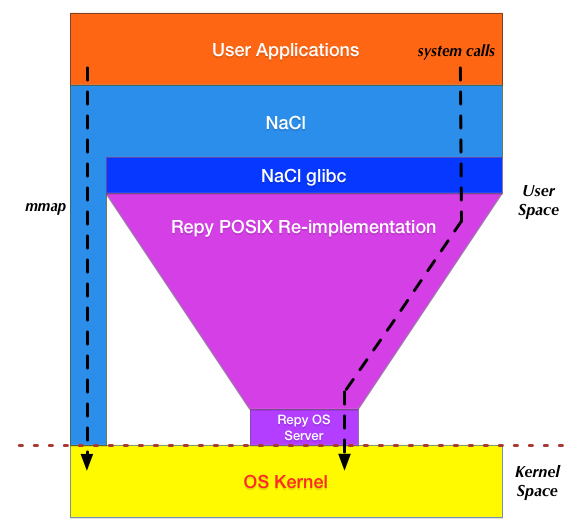
\includegraphics[width=1.0\columnwidth]{diagram/lind_architecture.png}
\caption{Architecture of Lind}
\label{fig:arch}
\end{figure}


%\par
%For a user application running in Lind, whenever a system call is needed, it will first go to NaCl glibc. Our modification on NaCl glibc will redirect the system call request to our Repy sandbox. In our Repy sandbox, a POSIX API will serve the system call request. Our POSIX interface is sufficient for most legacy applications, while only have minimal touch into the kernel. The design helps minimize the attack surface and effectively protects the kernel from being exploited. 


\par
To provide native computation and safe access to the system, Lind combines NaCl and Repy. Untrusted programs are run in NaCl, but access to all system resources is diverted to our Repy program. This program is responsible for accessing the system on behalf of the program, it is called the Lind Library OS. Our NaCl sandbox is built on top of our Repy sandbox. To service a system call in NaCl, a server routine marshals its arguments into a text string, and sends the call and the arguments to Repy sandbox. The Library OS then executes the appropriate system call, marshals the result and returns it back to NaCl. The result is eventually returned as the appropriate native type to the calling program. 


\par
Lind is designed to minimize its footprint within the trusted code base (TCB) of these two sandboxes. To achieve that, most of the Lind code is run from within the two sandboxes, the modifications to the sandboxes themselves (and therefore the TCB) was extremely small. 


\par
The dual-layer sandbox mechanism completes the achievement of the isolation design goals through two features. First, the dual-layer sandbox ensures that all code can modify only device state, interact with devices, or interact with the outside world through the new trusted operating system interface. Secondly, the customizability of the interface ensures that the system can only modify state, interact with devices, or interact with the world at a rate and in a manner specified for the application. For example, any attempt to send spam or execute a denial of service attack would trigger limits on resource consumption and/or allowable addressing, and would be prevented. 


\par
The dual-layer sandbox also makes the construction of Lind simpler. The complex part of Lind is the Library OS which runs in Repy. However, Python is a very powerful language, so it significantly simplified the construction of Lind. Even though Python is considered ``slow'' by some, the internals of an application in Lind are run in NaCl, a very high performance environment. This balances the performance of the system, with the ease of implementation and maintenance of the Library OS component of Lind. 


\par
Furthermore, this particular design and architecture for sandboxing ensures the programs are portable. Programs running inside Lind are written to work against a standard POSIX glibc interface. The Lind runtime is strictly user-level and designed to work on many different platforms including Linux, Mac OSX and Windows.


\par
Our sandbox also ensures performance isolation. It is used to limit resource consumption, both of computational resources (CPU, memory) and external resources (disk I/O and space, network bandwidth). The interposed system calls rate limit access and total consumption of each class of device on a configurable basis. CPU and memory limits are enforced on a per-process basis. 


\par
Finally, this kind of sandboxing ensures that the lightweight goal is met. Overhead for the Lind system is low because the sandbox only incurs overhead when there is a system call; Lind uses a native interface for execution, allowing CPU-and-memory-intensive applications to run at speeds that are equivalent to NaCl and near native speed. 


\par
Regarding our dual-layer sandbox architecture, one fundamental question is: are two sandboxes enough and necessary? Why do we only have two sandboxes? If sandboxing provides more security, why not sandbox Repy sandbox's TCB and get more security? The answer to that question is: the lowest level sandbox eventually must have some fundamental yet limited access to system resources, such as memory, storage, threads, etc. So having multiple sandboxes is not necessary, and two sandboxes in our design would be enough. But are two sandboxes indeed necessary? Why not just have one sandbox that solves everything? The answer is that the kernel interface is extremely rich and hard to protect. In order to have minimal tough into the kernel, as well as provide sufficient API for legacy applications, we need to have more than one sandbox to complete the job. One sandbox focuses on protecting the kernel and providing POSIX API, the other sandbox deals with executing applications efficiently. That is the reason for us to have at least two sandboxes.  


\par 
The key point in our design is to achieve safe re-implementation of OS functionalities. However, our safe re-implementation has limitations. There are a few functionalities that we currently cannot re-implement in our sandbox. Those functionalities include brk, mmap, and threads creation.